\subsubsection{Le gaborium}

\paragraph{Le dispositif}Le gaborium utilise également des \glspl{gabor} comme stimulus. Un écran rempli d'une multitudes de gabors de tailles et d'orientations différentes est montré
au sujet. Tous les distracteurs sont des gabors avec une direction et une vitesse de mouvement constante. La cible est un gabor dont la direction et la vitesse changent constamment.
Dans cette tâche, le sujet doit cliquer sur la cible avec la souris des qu'il l'aperçoit. La cible disparaît alors et une autre cible fait son apparition après un laps de temps
variable. L'œil droit du sujet est traqué à l'aide d'un eye tracker Eyelink. Il doit également appuyer sur la barre espace s'il sent qu'il n'est plus concentré sur la tâche de Gaborium.

\begin{figure}[H]
    \begin{center}
    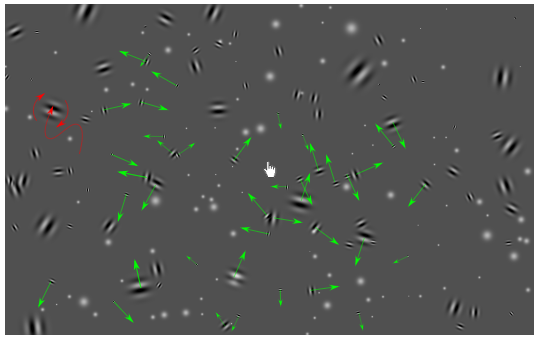
\includegraphics[width=11cm]{gaborium.png}
    \end{center}
    \caption{Gaborium avec les directions de certains gabors affichées}
\label{Gaborium}
\end{figure}

\paragraph{Traitement des données}Les données à observer pour l'analyse de l'attention sur la tâche sont les temps de réaction et la fréquence à laquelle le sujet appuie sur la barre
espace. La tâche ayant été créée récemment, elle n'est pas encore parfaite : peu de gens voire personne n'appuie sur la barre espace. Nous n'avons donc pas de données exploitables.
On a donc essayé d'enregistrer le mouvement des yeux ainsi que le diamètre pupillaire. Nous savons qu'il existe un lien entre ce diamètre et l'aspect émotionnel et attentionnel d'une
personne : plus le diamètre est grand et plus la personne est attentive. Néanmoins, on sait aussi que le diamètre pupillaire change aussi selon la luminosité. Dans les données, nous
avons donc des fluctuations rapides représentant le changement de luminosité entre le fond gris et les gabors noirs, et des fluctuations plus lentes représentant le niveau attentionnel
du sujet.